%
% ---------------------------------------------------
%
% Proyecto de Final de Carrera:
% Author: Adriano dos Santos Moreira <alu0101436784@ull.edu.es>
% Chapter: SYCL
% File: Cap3_SYCL.tex
%
% ----------------------------------------------------
%


\chapter{SYCL} \label{chap:SYCL}

In this chapter we will take a deep dive into the mechanisms and abstractions that the SYCL platform offers.

We chose \textit{Data Parallel C++} \cite{Reinders:2023:Data} as the baseline book to learn about SYCL.
It is a very recently published reference for this platform (first edition published in November 2020, second in October 2023) that also serves as an introduction to parallel programming, as it introduces the very basic concepts and builds on them in a beginner friendly manner.
On the other hand, SYCL Academy\footnote{\href{https://github.com/codeplaysoftware/syclacademy}{{SYCL Academy} \url{https://github.com/codeplaysoftware/syclacademy}}} fills the need for a more practical approach for an introduction to SYCL, offering a 20 lectures long tutorial, containing both lessons and exercises.

Based on the study of the mentioned sources, in the following sections we will cover the foundational ideas and procedures contained in the SYCL platform.

Nevertheless, this chapter does not aim to provide an exhaustive explanation of SYCL and its programming API.
For a deeper understanding, the interested reader is referred to the above references, also including the SYCL technical specification \cite{URL::SYCL-Specification}.

\section{What is SYCL?}

SYCL is a parallel focused abstraction layer created for C++. Although the idea of a mechanism that provides tools for parallelism existed for a long time, the unique trait of SYCL is that it attempts to define a uniform protocol for parallel execution.
In such a way, it allows for portable programmability across multiple vendors and platforms. Thus, bringing to existence a powerful tool which fulfils the following statement from \textit{Parallelizing the Standard Algorithms Library} \cite{Hoberock:2012:Parallelizing}:

\vspace{3mm}
\textit{``...standard and broadly-accessible functionality should be constructed to bridge the gap between the abundant parallelism implicit in many applications and the concurrent resources of the target architecture...''} 
\vspace{3mm}

This is a notable effort since these features were desired for almost a decade by the time SYCL 2020 was launched.

It is worth mentioning that SYCL has some similarities to OpenCL, sharing concepts and terminology like NDRanges and command queues (called just queues in SYCL).
In fact, when SYCL was created it was an abstraction layer only for OpenCL, and later it was expanded to support multiple back-ends in SYCL 2020.

Having stated what SYCL is, we will review a simple SYCL program that performs a scalar addition so we can grasp how a minimal SYCL operates.
In the first line of Listing \ref{listing:scalar-add} we have the inclusion of the SYCL header file.

\lstinputlisting[language=C++,style=cppstyle,caption={Scalar add example using the buffer/accessor model. \href{{https://github.com/AdrianoMoreira08/TFG-SYCL/blob/main/sycl-examples/scalar_add.cc}}{\textit{See on Github}}.},label={listing:scalar-add}]{listings/scalar_add.cc}

This code performs the sum of \texttt{summand\_a} and \texttt{summand\_b}, writing the result in the \texttt{result} variable.
On line 6 we have the key object of any SYCL program, the queue.
It allows for communication between host and device and execute various operations.
Lines 8-10 define buffers to manage the previously stated data.

Then we have a call to \texttt{submit} in line 12, which schedules a \textit{command group} to be executed.
Which is, to simplify, a set of arbitrary code and a kernel execution call.
This is the first step to get actual kernel code executing on a device.

Inside this command group there are three \textit{accessors}, which grant access to the buffers within the kernel.
On lines 17-19 there is the kernel definition and invocation.

In the next sections of this chapter we will cover the details and unexplained elements of this example.

\section{The Queue}

Queues\footnote{\url{https://registry.khronos.org/SYCL/specs/sycl-2020/html/sycl-2020.html\#sec:interface.queue.class}} are the main piece of action in SYCL.
They allow the host program to communicate with an underlying device or devices.
An instance of a queue is connected to one device and can execute different operations concerning the device itself and between host and device.
Note that multiple queues can be bound to the same device but one queue is only bound to a single device.
Another point to mention is that the SYCL host program can be executed on any type of physical device as long as it supports C++17, although is often going to be executed on a CPU.

\subsection{Task Graph}

SYCL organizes the work to be performed using a dependency graph.\footnote{\url{https://registry.khronos.org/SYCL/specs/sycl-2020/html/sycl-2020.html\#sec:command-groups-exec-order}}
Each node of the graph represents a unit of work, and the edges between them symbolize either custom or automatically set dependencies, as the example shown in Figure \ref{fig:dependency-graph}.

\begin{figure}[H]
    \centering
    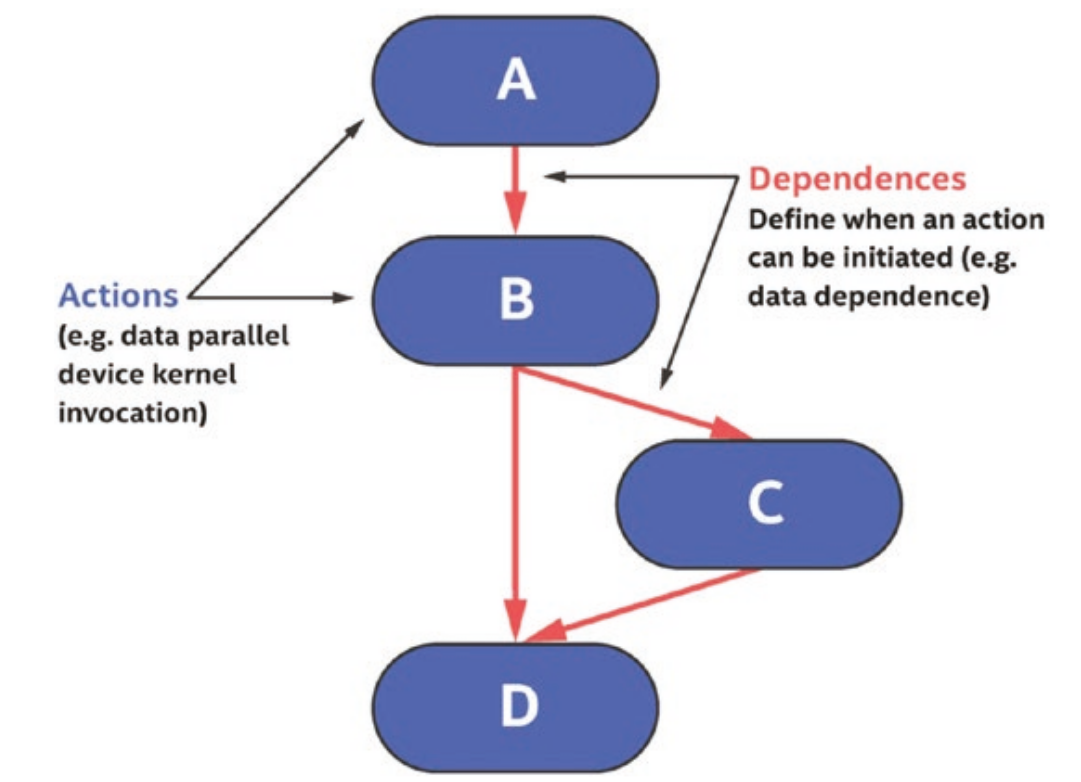
\includegraphics[width=0.7\linewidth]{images/dependency-graph.png}
    \caption{Dependency graph example. \textit{Image From Data Parallel C++} \cite{Reinders:2023:Data}}
    \label{fig:dependency-graph}
\end{figure}

With this structure, it is easy to determine which actions come next, as well as ensuring that the work is safe to execute.
SYCL automatically sets dependencies when working with the buffer/accessor model, as it provides the runtime with information regarding the use of the data present in the buffers.
On the other hand, in the Unified Shared Memory (USM) model, which is based on memory pointers, there is automatic data dependency management only when using certain types of pointers.
It is also possible to create dependencies manually.

\subsection{Device Selection}

When creating a queue, a device is assigned to it.
If nothing is specified, the runtime will select a device without taking into consideration the program needs, which can result in a device selection lacking the features the code requires.
SYCL will always guarantee that at least one device is available.

There are methods\footnote{\url{https://registry.khronos.org/SYCL/specs/sycl-2020/html/sycl-2020.html\#sec:device-selector}} to choose a specific device or with specific characteristics.
The functions \texttt{cpu\_selector\_v} (as seen on Listing \ref{listing:cpu-selector}) and \texttt{gpu\_selector\_v}, among others, are built-in selectors that can be passed as a parameter to the queue constructor to request for a certain type of device.
If device selection fails, the selector throws a \texttt{runtime\_error} exception.
\pagebreak

\lstinputlisting[language=C++,style=cppstyle,caption={Using a CPU selector. \href{{https://github.com/AdrianoMoreira08/TFG-SYCL/blob/main/sycl-examples/cpu_selector.cc}}{\textit{See on Github}}.},label={listing:cpu-selector}]{listings/cpu_selector.cc}

A more specific approach to device selection can be done by stating \textit{device aspects} using the \texttt{aspect\_selector} function, which tries to find a device that meets the declared aspects.

There is a list of standard aspects that can be requested, some of them include: \texttt{gpu}, \texttt{host\_debuggable} and \texttt{usm\_device\_allocations}.

There is an even more precise method to select a device.
Similarly to the built-in selectors, we can create a custom callable object or function that gives a score to each device.
It is an arbitrary procedure, so any technique can be used to calculate the score.
A good approach may be to use the \texttt{get\_info()} function template to retrieve data related to the device and calculate a score based on it.

\subsection{Errors and Exceptions}

When an error occurs in SYCL, it is handled through an exception.\footnote{\url{https://registry.khronos.org/SYCL/specs/sycl-2020/html/sycl-2020.html\#sec:interface.queue.errors}}
There are two types of errors:
\begin{itemize}
    \item \textbf{Asynchronous}, which result in exceptions thrown by the SYCL scheduler and may happen on a device or when trying to launch work on a device.
    \item \textbf{Synchronous} that occur when an error condition can be identified when the host program executes an operation.
\end{itemize}
\pagebreak
\lstinputlisting[language=C++,style=cppstyle,caption={Synchronous and asynchronous error handling procedures. \href{{https://github.com/AdrianoMoreira08/TFG-SYCL/blob/main/sycl-examples/error_handling.cc}}{\textit{See on Github}}.},label={listing:error-handling}]{listings/error_handling.cc}

The way synchronous and asynchronous errors are handled differ.
A synchronous error can be caught within the host program in a similar way to the example of Listing \ref{listing:error-handling}, where the try-catch block handles the situation when something goes wrong.

On the other hand, asynchronous errors are passed on to an \textit{asynchronous handler}, a function that is called at specific points in the code.
This function can be created manually to customize its behaviour and we can find an example in line 6 of Listing \ref{listing:error-handling}.
It can be arbitrarily called using \texttt{queue::throw\_asynchronous()} (or other similar methods) and is automatically called when a queue or context is destroyed.

\section{Buffer/accessor Model} \label{sec:buffer-accessor}

Buffers are abstractions that represent an object or collection of objects.\footnote{\url{https://registry.khronos.org/SYCL/specs/sycl-2020/html/sycl-2020.html\#subsec:buffers}}
The type of the objects they manage can vary from C++ scalar types, SYCL vectors, structures and user-defined types that comply with the notion of being \textit{device copyable}, which we will not go into in detail here.

By themselves, buffers do not hold the data, they simply represent it.
This model is based on the interaction with the buffers and stating the actions to be performed on them.\footnote{\url{https://registry.khronos.org/SYCL/specs/sycl-2020/html/sycl-2020.html\#subsec:accessors}}
With this information, the runtime schedules all the necessary data transactions to perform the task.

\lstinputlisting[language=C++,style=cppstyle,caption={Scalar add example using the buffer/accessor model. \href{{https://github.com/AdrianoMoreira08/TFG-SYCL/blob/main/sycl-examples/scalar_add.cc}}{\textit{See on Github}}.},label={listing:scalar-add-2}]{listings/scalar_add.cc}

We will take the first SYCL program presented at the beginning of the chapter to explain the usage of the buffer/accessor model.
In lines 8-10 of Listing \ref{listing:scalar-add-2}, we define the buffers by passing a reference to the original variable and a \texttt{range} indicating how many items does the variable hold (if it was an array, its size would match the range).

To use the buffers we use \texttt{accessors}, located in lines 13-15.
To be created, they just need the buffer that is being accessed and the handler, as the data type of the buffers is deduced.
Then we can use the accessors as if they were the original variables.

SYCL provides data consistency and is in charge of moving the information to the places it is used when using the buffer/accessor model.
For further optimization, we can communicate to the runtime what we are planning to do with the data.
To do this, we can add a third parameter to the definition of the accessors, stating the type of operation that is going to take place, the \textit{access mode}.
In the case of the example, it would make sense to mark \texttt{in\_a} and \texttt{in\_b} as \texttt{sycl::read\_only} and the \texttt{out\_r} buffer as \texttt{sycl::write\_only}.
This example was not written in this way to prioritise readability, as this is the first contact with the model.

Finally, we need to address line 7, which references the buffer's scope.
Getting a buffer out of scope (destroying it) is one of the simplest ways of copying the data managed by the buffer back to the original variable.
After line 21, the scope of the buffers ends, resulting in a copy from wherever the most recent version of the information is to its original source.
This is one of a handful of methods that exists to retrieve information from a buffer, which include forcing an update of the original variables without destroying the buffer and using a \texttt{host\_accessor} to access the data from the host.

\section{Unified Shared Memory Model}

USM\footnote{\url{https://registry.khronos.org/SYCL/specs/sycl-2020/html/sycl-2020.html\#sec:usm}} is a pointer-based model that leverages devices that support a unified virtual address space, meaning that a host memory pointer created using USM serves as a valid pointer address in the device.
There are three types of memory allocation:
\begin{itemize}
    \item \texttt{device}: Allocation happens in device memory.
    Can be directly accessed from the device but has to be explicitly copied to the host to be accessed from there.
    \item \texttt{host}: Host allocated memory that can also be accessed from the device without an explicit copy.
    To retrieve this data from the device, it is streamed over a bus rather than copied.
    \item \texttt{shared}: Similarly to a \texttt{host} allocation, the information can be accessed from both the host and device.
    The difference is that data can migrate back and forth between host and device.
\end{itemize}
\pagebreak
\lstinputlisting[language=C++,style=cppstyle,caption={Multiple scalar additions using the USM model. \href{{https://github.com/AdrianoMoreira08/TFG-SYCL/blob/main/sycl-examples/usm_scalar_add.cc}}{\textit{See on Github}}.},label={listing:usm-scalar-add}]{listings/usm_scalar_add.cc}

The USM model offers implicit data movement using \texttt{host} or \texttt{shared} allocations, while also giving the possibility to use explicit data movement through \texttt{device} allocations.
On Listing \ref{listing:usm-scalar-add} we can see a parallel scalar addition using \texttt{shared} memory.
We observe that memory access is pretty straightforward, just as if we were using regular C++ arrays.
Although this is simple, behind the scenes there are additional schedules in place to deliver the information.
In the last lines of Listing \ref{listing:usm-scalar-add}, we free the memory using SYCL's \texttt{free} function.

\section{Work Submission}

A host program can schedule memory management tasks as well as kernel execution tasks.\footnote{\url{https://registry.khronos.org/SYCL/specs/sycl-2020/html/sycl-2020.html\#\_queue\_interface}}
These operations will always be encapsulated within a command group, which is then submitted to the queue.

The submitted work will be organized into the task graph and executed when possible (after meeting the dependency requirements) in an arbitrary order or even may be executed in parallel.
This is the behaviour of \textit{out-of-order} queues and the default behaviour of queues.
It is possible to create an \textit{in-order} queue by passing the \texttt{in\_order} queue property to the queue constructor, which will execute tasks one at a time.

\vspace{5mm}
\textsl{\textbf{{Command Group}}}
\vspace{2mm}

A command group (CG) is a lambda expression or function object \cite{Jarvi:2010:CLE} that defines all the necessary elements and details of a task.
It takes a SYCL \textit{handler} reference as an argument, which is used to configure the CG and has methods to perform task actions.
There are two categories of code within a CG:
\begin{itemize}
    \item \textbf{Host code}: This is arbitrary code that runs on the host, which executes immediately upon submitting the CG.
    It is used to define buffer accessors and other node dependency configuration, such as \texttt{depends\_on()} calls to manually set up dependencies.
    The runtime then uses all the information supplied to determine the relationships between the tasks on the task graph and places the new task where it belongs with the corresponding edges.
    \item \textbf{Action}: Can be either a kernel to execute on the device or an explicit memory operation.
    It is not required to write an action, but there is a limit to one action per CG.    
\end{itemize}

Although the host code section of a CG can hold any arbitrary host code, it is recommended to \textbf{only} write the necessary code to set up the dependencies.

Also note that \texttt{depends\_on()} calls take an event or events as arguments.
Those events represent already submitted tasks and can be obtained from the return object of a submit call.

\subsection{Memory Operations}

Memory transaction operations can vary depending on the context of our code.
For example, the \texttt{memcopy()} function allows for explicit data movement, which can be used in combination with the explicit version of the USM model to handle memory ourselves.
Other memory related functionalities include:
\begin{itemize}
    \item \texttt{memset()}: Fills a memory region with the same unsigned char value.
    \item \texttt{fill()}: Fills a memory region with the same arbitrary object.
    \item \texttt{update\_host()}: Updates the memory object referred by an accessor in host to its latest version.
\end{itemize}

\subsection{Basic Kernels}

There are two types of kernels that can be submitted to the dependency graph.
The simplest of them is \texttt{single\_task()}\footnote{\url{https://registry.khronos.org/SYCL/specs/sycl-2020/html/sycl-2020.html\#\_single\_task\_invoke}}, which executes a single instance of a device function.
On the other hand, we can launch multiple instances of device code using \texttt{parallel\_for()}, which can be executed with different combinations of work sizes.

\lstinputlisting[language=C++,style=cppstyle,caption={Multiple scalar additions using \texttt{parallel\_for()}. \href{{https://github.com/AdrianoMoreira08/TFG-SYCL/blob/main/sycl-examples/usm_scalar_add.cc}}{\textit{See on Github}}.},label={listing:scalar-add-parallel-for}]{listings/usm_scalar_add.cc}

The scalar addition presented earlier serves as a fitting example.
In Listing \ref{listing:scalar-add-parallel-for}, we present an addition performed for every element of the summand arrays.
\pagebreak
\subsection{NDRange}

A more granular method of defining a kernel is by using an NDRange, which offers an execution space that can be broken down into different groups, as we can observe in Figure \ref{fig:ndrange}.

\begin{figure}[H]
	\centering
	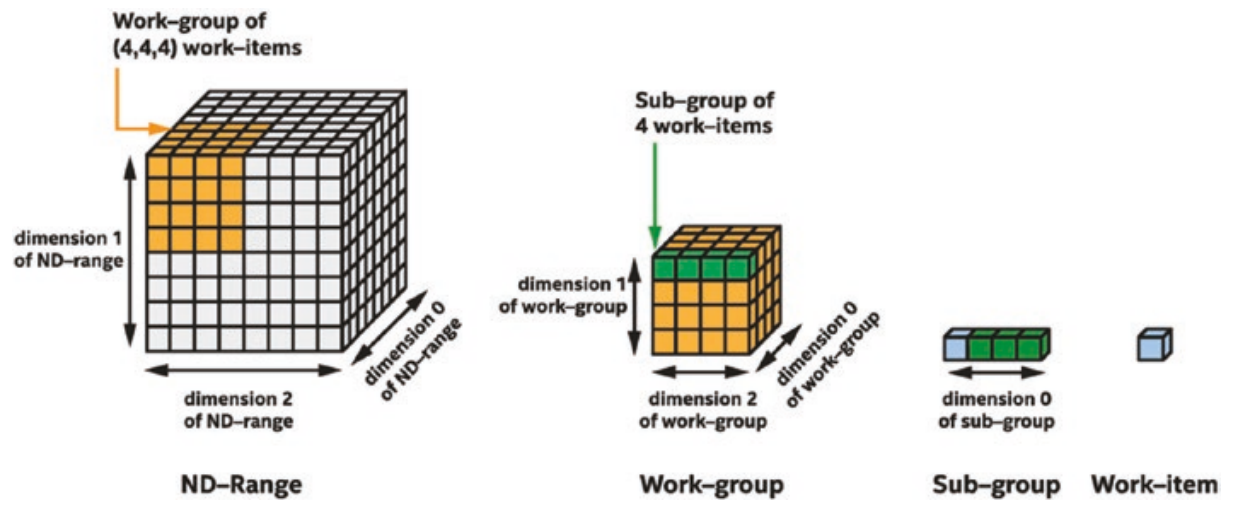
\includegraphics[width=\linewidth]{images/nd_range.png}
	\caption{Dissection of an NDRange. \textit{From Data Parallel C++} \cite{Reinders:2023:Data}.}
	\label{fig:ndrange}
\end{figure}

This coarse-grained structure enables the application of various strategies within the index space, allowing for the implementation of work-group oriented algorithm designs.
These include strategies like memory tiling, which take advantage of work-group synchronization procedures.
